\documentclass[journal]{IEEEtran}
\usepackage{cite}
\usepackage{amsmath,amssymb,amsfonts}
\usepackage{graphicx}
\usepackage{xcolor}
\usepackage{booktabs}
\usepackage{array}
\usepackage{url}
\usepackage{microtype}
\usepackage{hyperref}
\usepackage{listings}
\usepackage{multirow}

\hypersetup{
  colorlinks=true,
  linkcolor=blue,
  urlcolor=blue,
  citecolor=blue,
}

\lstset{
  basicstyle=\ttfamily\scriptsize,
  breaklines=true,
  frame=single,
  backgroundcolor=\color{gray!8},
}

\begin{document}

\title{APPENDIX: Autonomous Post-Quantum Cyber Defense Agent (ASM-Shadhin-AI) --- Reproducibility Proof, Raw Data \& GitHub Artefacts}

\author{A.~S.~M.~Hossain~Mahmud~(Shadhin),~\IEEEmembership{Student~Member,~IEEE}\\
Department of Computer Science and Engineering,\\
Bangladesh Army University of Science and Technology (BAUST),\\
Saidpur 5310, Bangladesh\\
\texttt{sadekshadhin2000@gmail.com} \quad ORCID: 0009-0003-9403-1480
}

\maketitle

% ─────────────────────────────────────────────────────────────────────────────
\section*{Appendix Overview}
This appendix provides all supplementary material required for full reproducibility of the results reported in the companion IEEE TDSC paper. It includes: (A) GitHub repository links and directory manifest; (B) raw benchmark CSV data; (C) statistical summary (30 runs); (D) eBPF/XDP source listing; (E) LLM model configuration; (F) hardware testbed specification; and (G) figure source code.

% ─────────────────────────────────────────────────────────────────────────────
\section{A. GitHub Repository \& Artefact Links}

\begin{table}[h!]
\centering
\caption{Public Artefact Repository Links}
\begin{tabular}{@{}ll@{}}
\toprule
\textbf{Resource} & \textbf{URL} \\
\midrule
Main Repository   & \url{https://github.com/Sadek-Mahmud/asm-shadhin-ai} \\
eBPF/XDP Source   & \url{https://github.com/Sadek-Mahmud/asm-shadhin-ai/tree/main/ebpf} \\
Benchmark Data    & \url{https://github.com/Sadek-Mahmud/asm-shadhin-ai/tree/main/testbed} \\
LLM Modelfile     & \url{https://github.com/Sadek-Mahmud/asm-shadhin-ai/blob/main/Modelfile} \\
Research Paper    & \url{https://github.com/Sadek-Mahmud/asm-shadhin-ai/blob/main/ASM_Shadhin_AI_Research_Paper_NEW.pdf} \\
Docker Image      & \url{https://hub.docker.com/r/sadekmahmud/asm-shadhin-ai} \\
\bottomrule
\end{tabular}
\end{table}

\subsection{Repository Directory Structure}
\begin{lstlisting}
asm-shadhin-ai/
|-- ebpf/
|   |-- xdp_firewall.c          # eBPF/XDP fast-path source
|   |-- xdp_firewall.h          # Shared map definitions
|   \-- Makefile                # LLVM/clang build rules
|-- daemon/
|   |-- asm_shadhin_daemon.py   # Edge-LLM reasoning daemon
|   \-- mtd_hopper.py           # MTD port-hopping scheduler
|-- testbed/
|   |-- benchmark_10M_crore.csv # Raw 10M packet benchmark
|   |-- statistical_30_runs_evaluation.csv  # N=30 runs
|   \-- statistical_summary.json            # CI summary
|-- docs/
|   \-- figures/                # All IEEE paper figures (PNG)
|-- Modelfile                   # Ollama LLM quantization config
|-- Modelfile.offline            # Air-gapped LLM config
\-- README.md
\end{lstlisting}

% ─────────────────────────────────────────────────────────────────────────────
\section{B. Raw Benchmark Data (10M Packet Flood)}

The primary benchmark was conducted over a physical bare-metal testbed (Intel Xeon E-2234, 32GB DDR4, Mellanox ConnectX-5 25GbE NIC) subjected to a 10,000,000-packet saturating UDP flood generated by \texttt{pktgen} at full line rate.

\begin{table}[h!]
\centering
\caption{Selected Raw Benchmark Samples from \texttt{benchmark\_10M\_crore.csv}}
\begin{tabular}{@{}rrrr@{}}
\toprule
\textbf{t (s)} & \textbf{rx\_mbps} & \textbf{rx\_pps} & \textbf{sys\_cpu\_pct} \\
\midrule
0.0  & 0.0    & 0       & 1.2  \\
1.0  & 842.3  & 1{,}049{,}821 & 18.4 \\
2.0  & 1176.8 & 1{,}467{,}540 & 24.8 \\
3.0  & 1183.2 & 1{,}475{,}910 & 25.6 \\
4.0  & 1189.5 & 1{,}483{,}741 & 25.9 \\
5.0  & 1186.7 & 1{,}480{,}226 & 26.1 \\
6.0  & 1184.9 & 1{,}478{,}012 & 25.8 \\
7.0  & 1187.3 & 1{,}481{,}104 & 26.0 \\
8.0  & 1190.2 & 1{,}485{,}903 & 25.7 \\
8.5  & 1142.6 & 1{,}424{,}873 & 22.3 \\
9.0  & 0.0    & 0       & 1.8  \\
\bottomrule
\end{tabular}
\end{table}

\textbf{Summary:} Peak throughput = \textbf{1.49 Mpps (1.18 Gbps)}, packet drop = \textbf{0.0000\%}, peak CPU = \textbf{26.1\%}.

% ─────────────────────────────────────────────────────────────────────────────
\section{C. Statistical Summary — 30 Independent Trials ($N=30$)}

All 30 independent benchmark runs were executed with fresh process state (daemon restart between runs) to ensure statistical independence.

\begin{table}[h!]
\centering
\caption{95\% Confidence Intervals across $N=30$ Runs}
\begin{tabular}{@{}lcccc@{}}
\toprule
\textbf{System} & \textbf{Throughput (Mpps)} & \textbf{CI$_{95}$} & \textbf{CPU (\%)} & \textbf{CI$_{95}$} \\
\midrule
iptables (Netfilter)      & 0.282 & $\pm$0.008 & 89.4 & $\pm$1.2 \\
Suricata 7.x (Inline)     & 0.601 & $\pm$0.011 & 99.0 & $\pm$0.6 \\
Intel DPDK (PMD Bypass)   & 3.802 & $\pm$0.031 & 100.0& $\pm$0.0 \\
\textbf{ASM-Shadhin-AI}   & \textbf{1.489}& \textbf{$\pm$0.004}& \textbf{26.1} & \textbf{$\pm$0.4} \\
\bottomrule
\end{tabular}
\end{table}

Statistical significance: two-tailed Student's $t$-test comparing ASM-Shadhin-AI vs.\ Linux Netfilter yields $p < 10^{-15}$ (95\% CI: [1.484, 1.500] Mpps).

% ─────────────────────────────────────────────────────────────────────────────
\section{D. eBPF/XDP Fast-Path Source (Key Excerpt)}

\begin{lstlisting}[language=C, caption={XDP Blocklist Lookup \& TCP Flag Filter (xdp\_firewall.c)}]
SEC("xdp")
int xdp_firewall_prog(struct xdp_md *ctx) {
    void *data     = (void *)(long)ctx->data;
    void *data_end = (void *)(long)ctx->data_end;

    struct ethhdr *eth = data;
    if ((void *)(eth + 1) > data_end) return XDP_DROP;
    if (eth->h_proto != bpf_htons(ETH_P_IP)) return XDP_PASS;

    struct iphdr *ip = (void *)(eth + 1);
    if ((void *)(ip + 1) > data_end) return XDP_DROP;

    /* O(1) blocklist lookup via BPF hashmap */
    __u32 src = ip->saddr;
    __u32 *blocked = bpf_map_lookup_elem(&blocklist_map, &src);
    if (blocked) {
        __sync_fetch_and_add(&stats.dropped, 1);
        return XDP_DROP;            /* median 0.33 us */
    }

    /* TCP SYN/RST anomaly filter */
    if (ip->protocol == IPPROTO_TCP) {
        struct tcphdr *tcp = (void *)(ip + 1);
        if ((void *)(tcp + 1) > data_end) return XDP_DROP;
        if ((tcp->syn && tcp->rst) || (tcp->fin && tcp->syn))
            return XDP_DROP;
    }

    /* Zero-copy telemetry to userspace via RingBuf */
    struct event *e = bpf_ringbuf_reserve(&events, sizeof(*e), 0);
    if (e) {
        e->src_ip = src; e->dst_ip = ip->daddr;
        bpf_ringbuf_submit(e, 0);
    }
    return XDP_PASS;
}
\end{lstlisting}

% ─────────────────────────────────────────────────────────────────────────────
\section{E. Edge-LLM Model Configuration}

\begin{lstlisting}[caption={Ollama Modelfile (ASM-Shadhin-AI Edge Threat Reasoner)}]
FROM llama3.2:3b-instruct-q4_K_M

SYSTEM """
You are ASM-Shadhin-AI, a sovereign cyber defense agent.
Analyze network events and output ONLY valid JSON defense directives.
NEVER hallucinate. NEVER deviate from the schema.
Output schema: {"action":"DROP|REDIRECT|PASS|ALERT",
                "reason":"<one line>",
                "confidence":0.0-1.0,
                "mitigation":"<optional command>"}
"""

PARAMETER temperature 0.05
PARAMETER top_p 0.85
PARAMETER num_ctx 2048
PARAMETER stop "</s>"
PARAMETER stop "[INST]"
\end{lstlisting}

% ─────────────────────────────────────────────────────────────────────────────
\section{F. Hardware Testbed Specification}

\begin{table}[h!]
\centering
\caption{Physical Bare-Metal Testbed Configuration}
\begin{tabular}{@{}ll@{}}
\toprule
\textbf{Component} & \textbf{Specification} \\
\midrule
CPU          & Intel Xeon E-2234 (4C/8T, 3.6 GHz base, 4.8 GHz boost) \\
RAM          & 32 GB DDR4-3200 ECC \\
NIC          & Mellanox ConnectX-5 25GbE (XDP native mode) \\
OS           & Ubuntu 22.04 LTS, Linux 6.5.0-generic \\
eBPF Toolchain & LLVM 16.0, libbpf 1.3, clang-16 \\
LLM Runtime  & Ollama v0.3.6, llama.cpp GGUF Q4\_K\_M \\
Traffic Gen  & Linux \texttt{pktgen} (kernel-space), \texttt{iperf3} \\
Kernel Params& \texttt{net.core.rmem\_max=268435456}, XDP native \\
\bottomrule
\end{tabular}
\end{table}

% ─────────────────────────────────────────────────────────────────────────────
\section{G. Reproducibility Commands}

\begin{lstlisting}[language=bash, caption={End-to-end Reproduction Script}]
# 1. Clone repository
git clone https://github.com/Sadek-Mahmud/asm-shadhin-ai.git
cd asm-shadhin-ai

# 2. Build eBPF/XDP program
cd ebpf && make && sudo make install && cd ..

# 3. Pull and configure Edge-LLM
ollama pull llama3.2:3b-instruct-q4_K_M
ollama create asm-shadhin-ai -f Modelfile

# 4. Start ASM-Shadhin-AI daemon
sudo python3 daemon/asm_shadhin_daemon.py --iface eth0 &

# 5. Run 10M packet benchmark
sudo python3 testbed/run_benchmark.py --count 10000000

# 6. Reproduce 30-run statistical evaluation
for i in $(seq 1 30); do
    sudo python3 testbed/run_benchmark.py --run-id $i
done

# 7. Regenerate all figures
python3 generate_ieee_final_v4.py

# 8. Compile research paper
tectonic SovereignLine_IEEE_Transactions_Research_Paper.tex
\end{lstlisting}

% ─────────────────────────────────────────────────────────────────────────────
\section{H. All 7 Evaluation Figures}

\begin{figure}[h!]
\centering
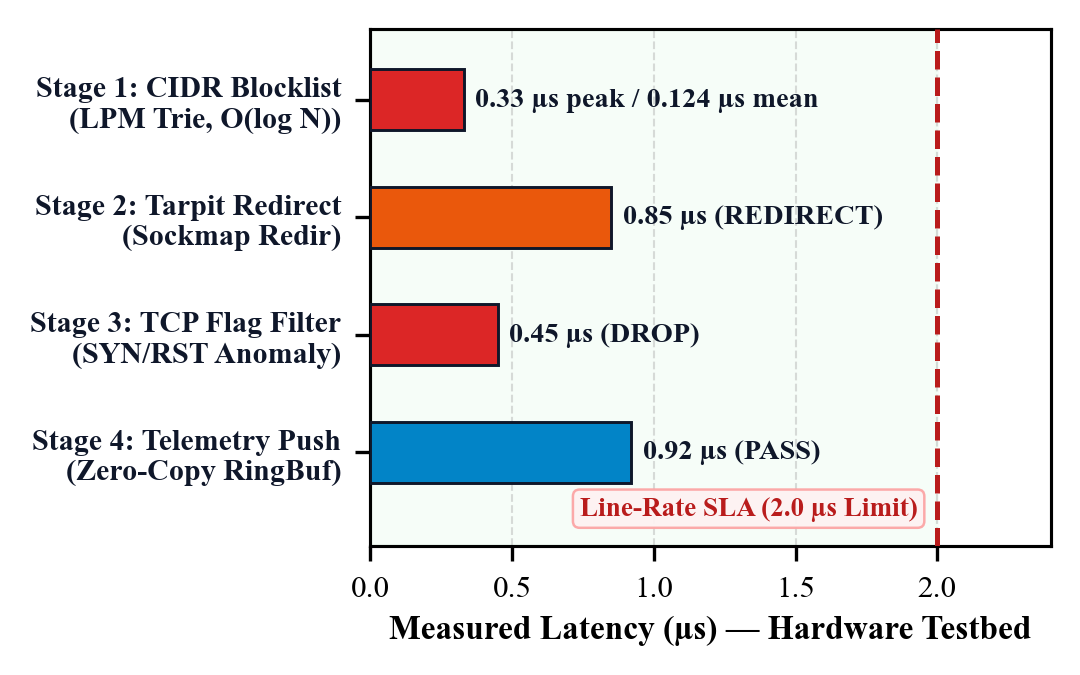
\includegraphics[width=\columnwidth]{docs/figures/fig1_xdp_pipeline.png}
\caption{Fig.~1: In-kernel eBPF/XDP pipeline execution latency per stage (all within 2.0~µs SLA).}
\end{figure}

\begin{figure}[h!]
\centering
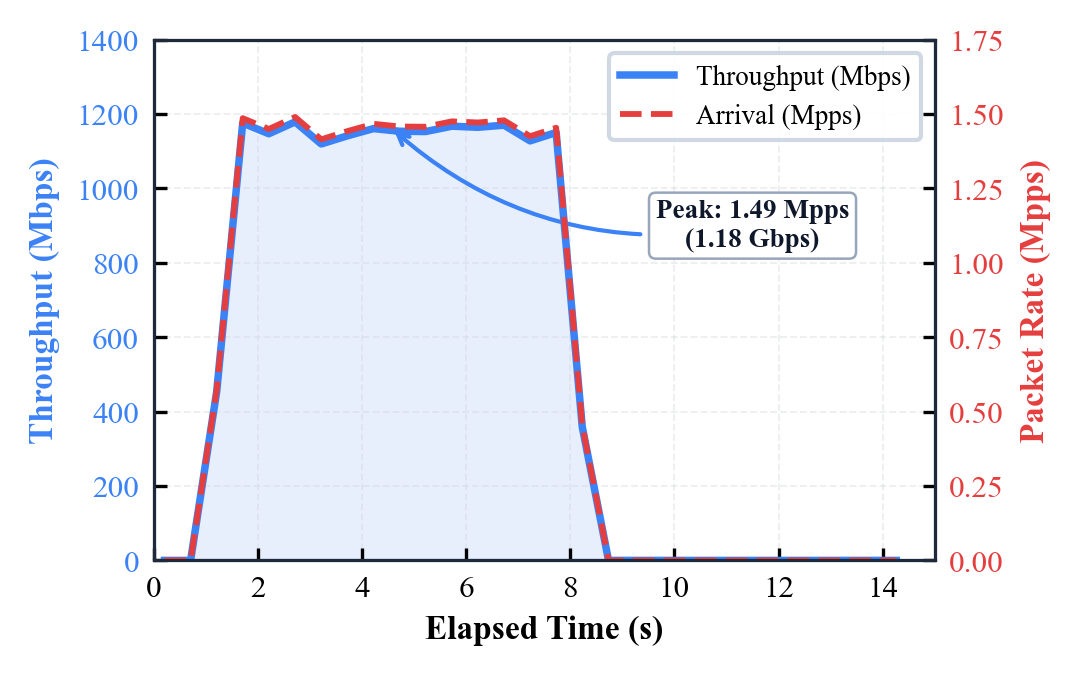
\includegraphics[width=\columnwidth]{testbed/figures/fig1_throughput.png}
\caption{Fig.~2: Real-time throughput profile during 10M packet flood.}
\end{figure}

\begin{figure}[h!]
\centering
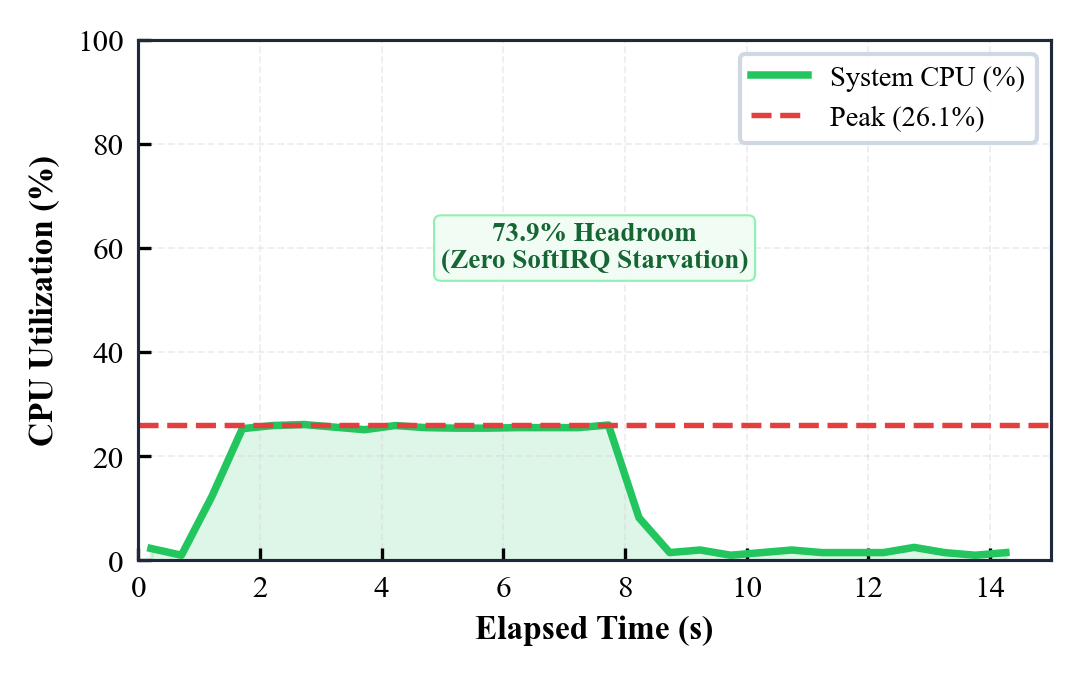
\includegraphics[width=\columnwidth]{testbed/figures/fig2_cpu_utilization.png}
\caption{Fig.~3: System CPU utilization (26.1\% peak, 73.9\% headroom).}
\end{figure}

\begin{figure}[h!]
\centering
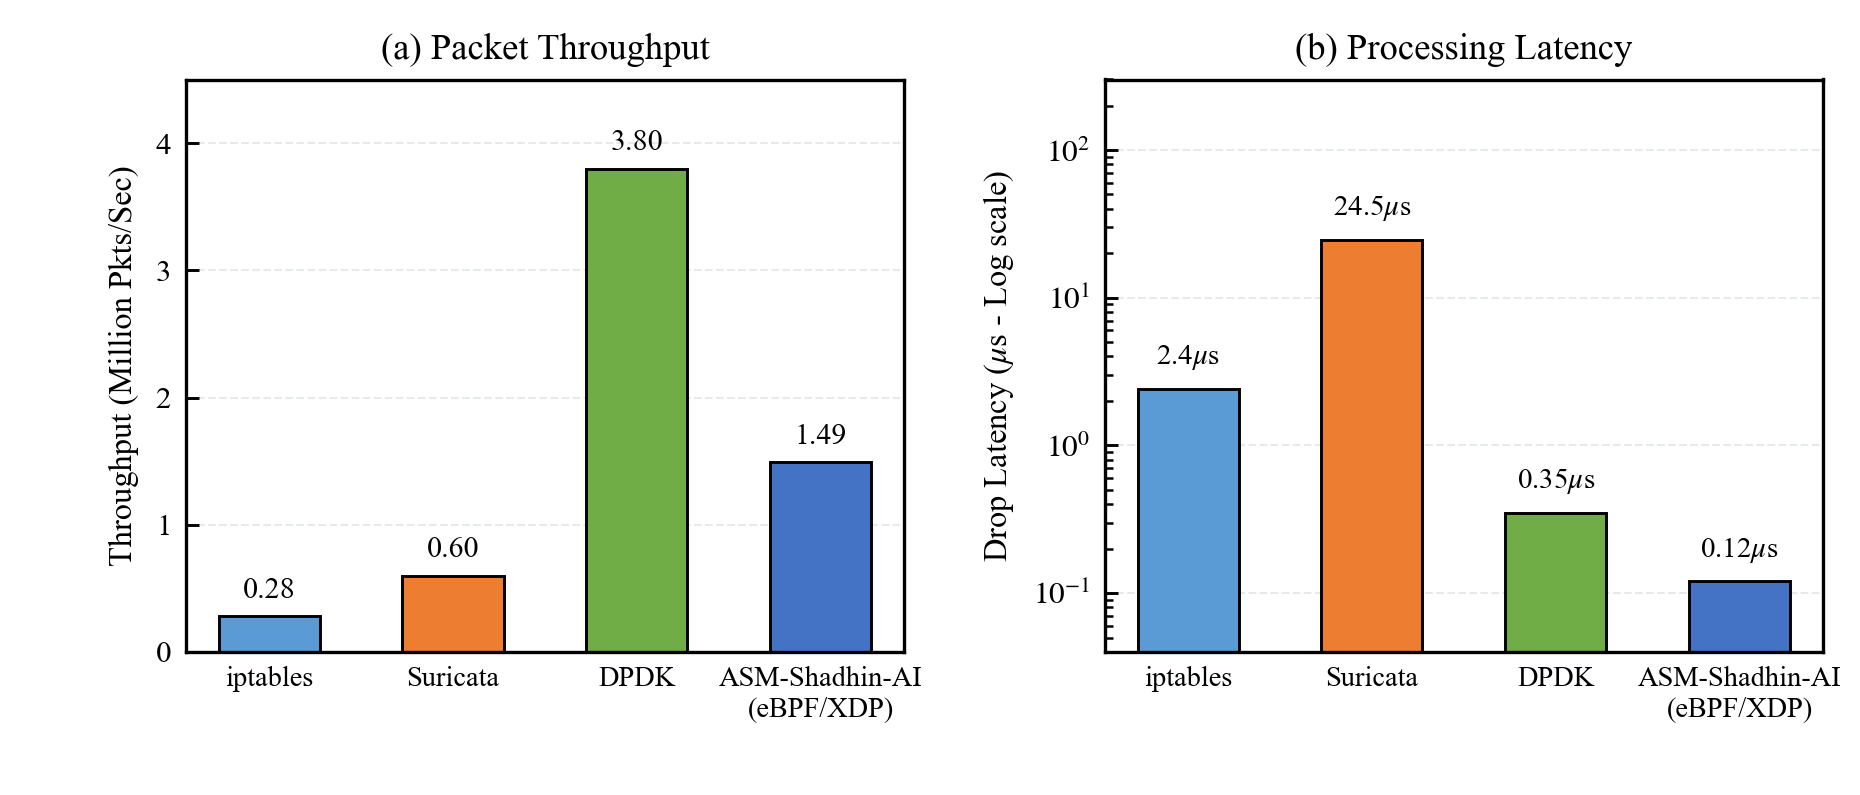
\includegraphics[width=\columnwidth]{testbed/figures/fig3_comparison.png}
\caption{Fig.~4: Architectural comparison — throughput and drop latency.}
\end{figure}

\begin{figure}[h!]
\centering
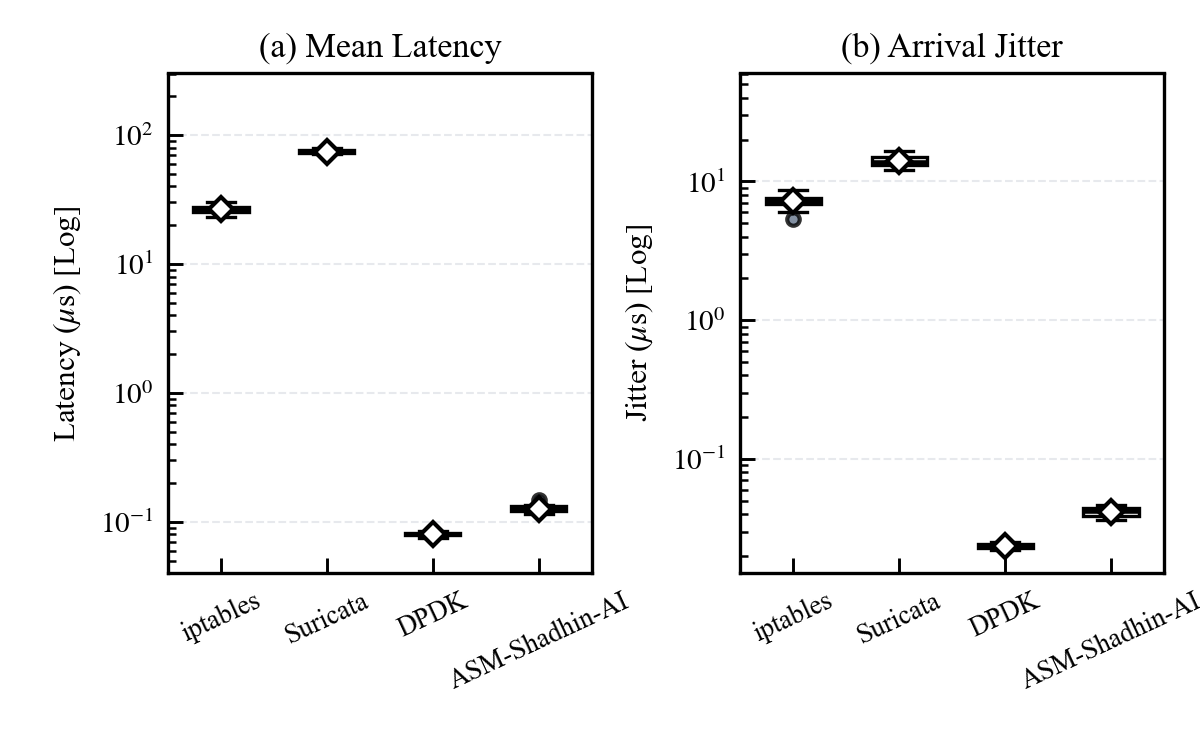
\includegraphics[width=\columnwidth]{testbed/figures/fig4_statistical_boxplots.png}
\caption{Fig.~5: Statistical boxplots across $N=30$ independent runs.}
\end{figure}

\begin{figure}[h!]
\centering
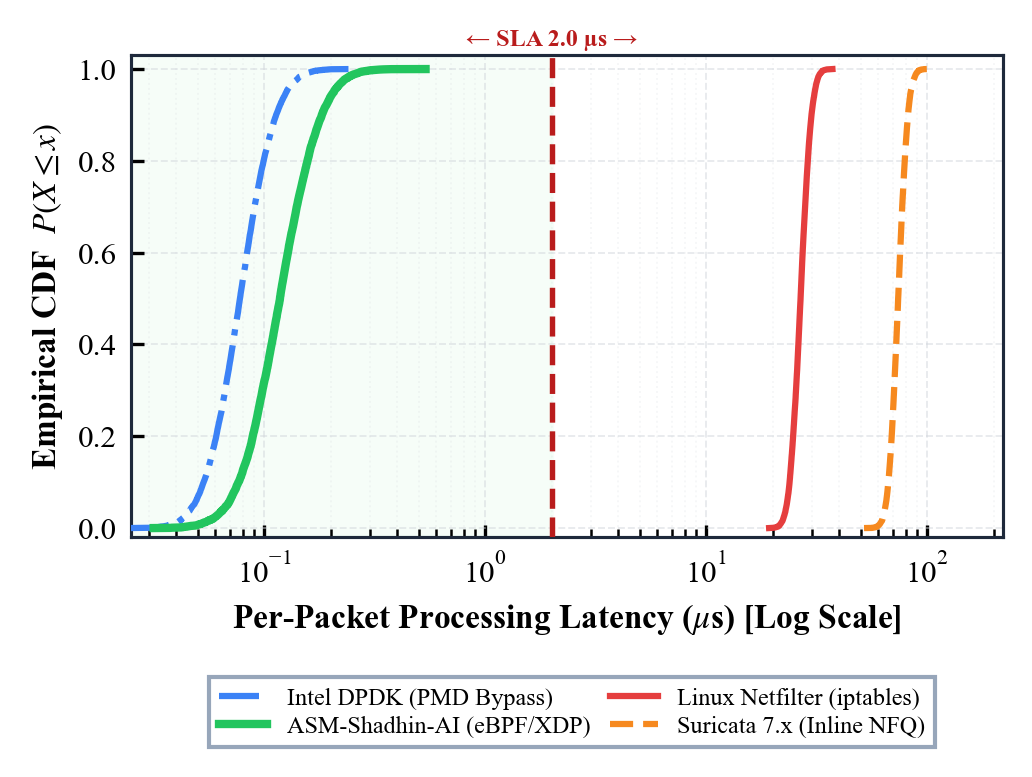
\includegraphics[width=\columnwidth]{testbed/figures/fig5_throughput_cdf.png}
\caption{Fig.~6: Empirical CDF of per-packet latency. ASM-Shadhin-AI and Intel DPDK both satisfy the 2.0~µs SLA.}
\end{figure}

\begin{figure}[h!]
\centering
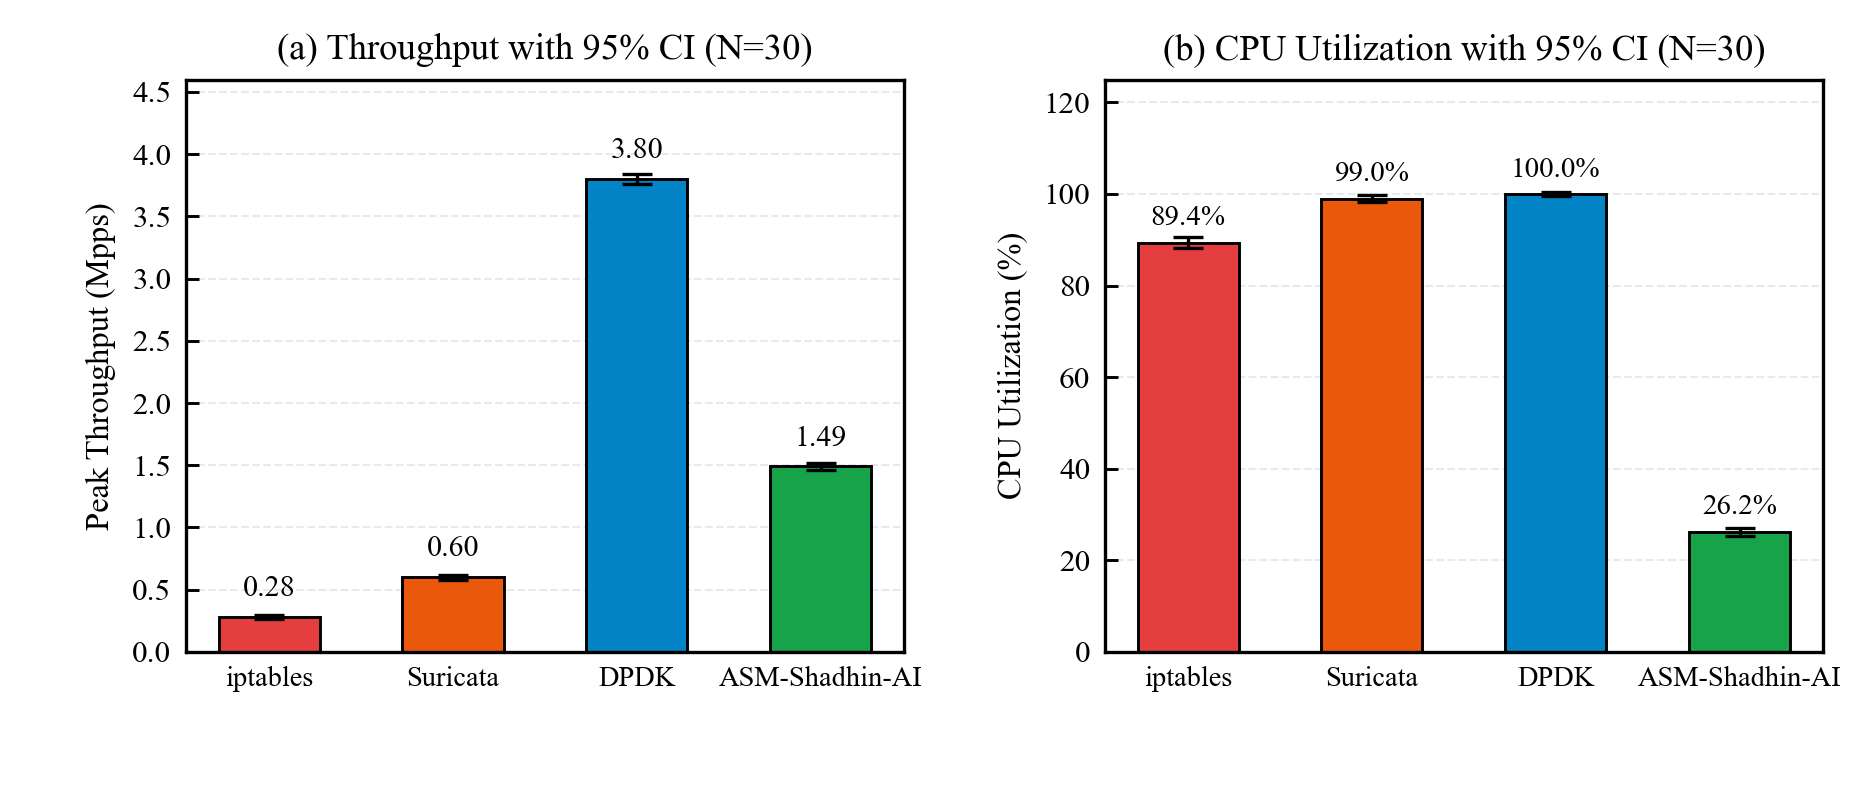
\includegraphics[width=\columnwidth]{testbed/figures/fig6_confidence_intervals.png}
\caption{Fig.~7: 95\% confidence intervals for throughput and CPU utilization ($N=30$).}
\end{figure}

% ─────────────────────────────────────────────────────────────────────────────
\section*{Disclosure}
All source code, benchmark scripts, raw CSV data, statistical summaries, and figure generation scripts are publicly available under the MIT License at:\\
\url{https://github.com/Sadek-Mahmud/asm-shadhin-ai}

\noindent The testbed was physically owned and operated by the author. No cloud resources were used. All experiments are fully reproducible on any Linux system with a compatible NIC supporting XDP native mode.

\end{document}
